\documentclass{article}
\usepackage[utf8]{inputenc}
\usepackage[T2A]{fontenc}
\usepackage[russian]{babel}
\usepackage{amsmath}
\usepackage{graphicx}

\begin{document}

\title{Практика 3}
\author{Ращупкин Е, Боков Е, Мишунин Н}
\maketitle

\section{Задача 1}
Кооперация «обработка события» EventHandling включает роли event, eventSource и eventListener. У одного источника событий может быть несколько слушателей.

\begin{itemize}
    \item Отобразите данную кооперацию на диаграмме классов.
    \item Реализуйте поведение менеджера событий с помощью кооперации EventHandling. Отразите участие классов EngineSource, EngineEvent, EngineListener, в кооперации EventHandling с назначенными ролями eventSource, event и eventListener при условии, что EngineSource может связан с несколькими экземплярами EngineListener.
    \item (*) Используя представление взаимодействия, постройте для данной кооперации модель поведения обработки события управляющим компонентом плеера. Экземпляр engineSource в роли eventsSource генерирует событие и уведомляет о нем подключаемые модули visPlugin и lyricsPlugin в роли eventsListener. Модуль lyricsPlugin обрабатывает событие, visPlugin игнорирует событие.
    \item Указание. Следует использовать диаграмму последовательности для отображения взаимодействия. На диаграмме показать линии жизни event, eventSource, visPlugin в роли eventListener и lyricsPlugin в роли eventListener. Указать вызов операции generateEvent в eventSource, указать вызов операции dispatch с параметром event от eventSource к visPlugin, который приводит к исполнению поведения, что отразить наличием спецификации выполнения. Далее, указать вызов dispatch от eventSource к lyricsPlugin, при получении которого не указана спецификация выполнения.
\end{itemize}

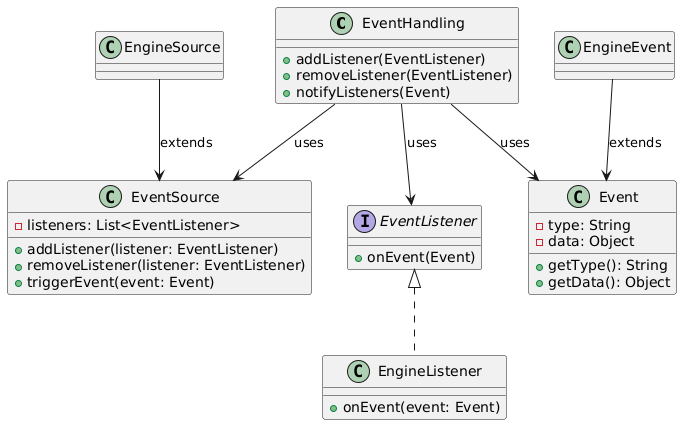
\includegraphics[width=\textwidth]{1_1.png}

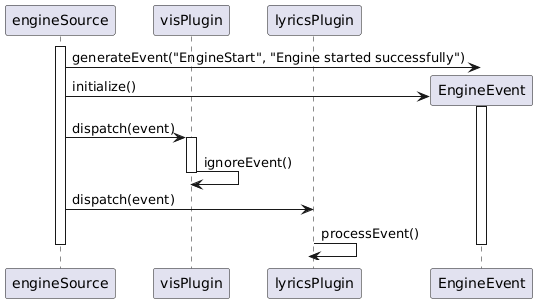
\includegraphics[width=\textwidth]{1_2.png}

\section{Задача 2}
Лифт Elevator состоит из кабины класса Cage, пульта управления класса ControlUnit и нескольких панелей вызова с этажа класса FloorControls. Соединитель между пультом управления и кабиной имеет тип cageWire, между пультом и панелями – floorWire. При этом пульт подсоединен к каждой панели индивидуально.

\begin{itemize}
    \item Добавьте в модель двигатель класса Engine как составную часть лифта. Двигатель связан с кабиной кабелем cable и с пультом схемой управления controls.
    \item Доработайте модель так, чтобы взаимодействие лифта с внешними классами происходило только через интерфейс кнопок кабины CageControls, управления лифтом Operations и интерфейсы вызова с этажей FloorButtons. Команды, принимаемые через интерфейсы, направляются на соответствующие части лифта.
    \item Укажите, что для работы лифту требуется подключение к электрической сети Power.
    \item Перечислите имена и типы всех элементов пространства имен класса Elevator.
    \item Чему соответствуют порты класса Elevator в коде реализации?
\end{itemize}

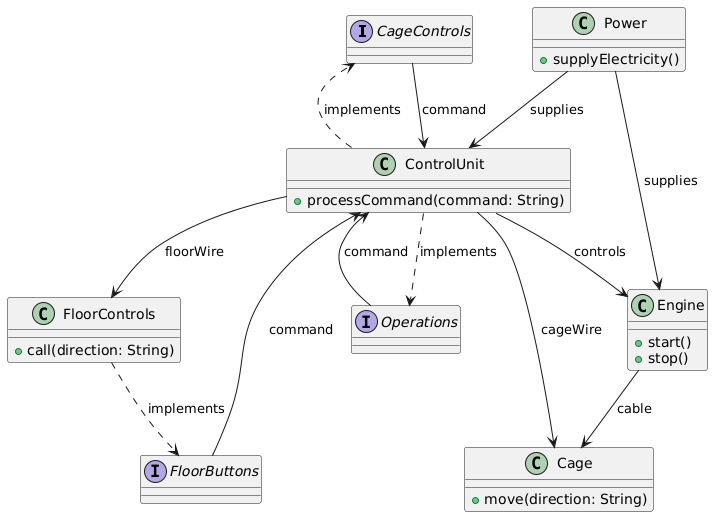
\includegraphics[width=\textwidth]{2.png}

\section{Задача 3}
Подсистема подготовки данных модуля морфологии MorphologyDPS состоит из базы данных Database, клиента для модификации данных DataClient, компонента экспорта Export и компилятора данных Compiler.
\begin{itemize}
    \item База данных предоставляет интерфейс изменения данных IMorphologyData и интерфейс экпорта данных IDataExport. Клиент требует для работы интерфейс изменения данных, в то время как компонент экспорта требует интерфейс экспорта данных. Компилятор не требует внешних интерфейсов, но неявно зависит от базы данных. Укажите в модели, как компоненты связаны между собой в подсистеме.
    \item Разместите базу данных на сервере MorphoDB, а остальные компоненты на компьютере лингвиста LinguistPlace.
    \item Уточните внутреннюю структуру компилятора следующим образом. Компилятор использует интерфейс IMorphology компонента MorphoModel. Сам компилятор состоит из парсера Parser, обработчика сообщений об ошибках Handler и сборщика модели Builder. Компоненты, реализующие парсер и сборку моделей, сообщают об ошибках через интерфейс IErrorHandler компонента Handler в составе компилятора. Сборщик модели компилятора требует внешний интерфейс IMorphology.
\end{itemize}

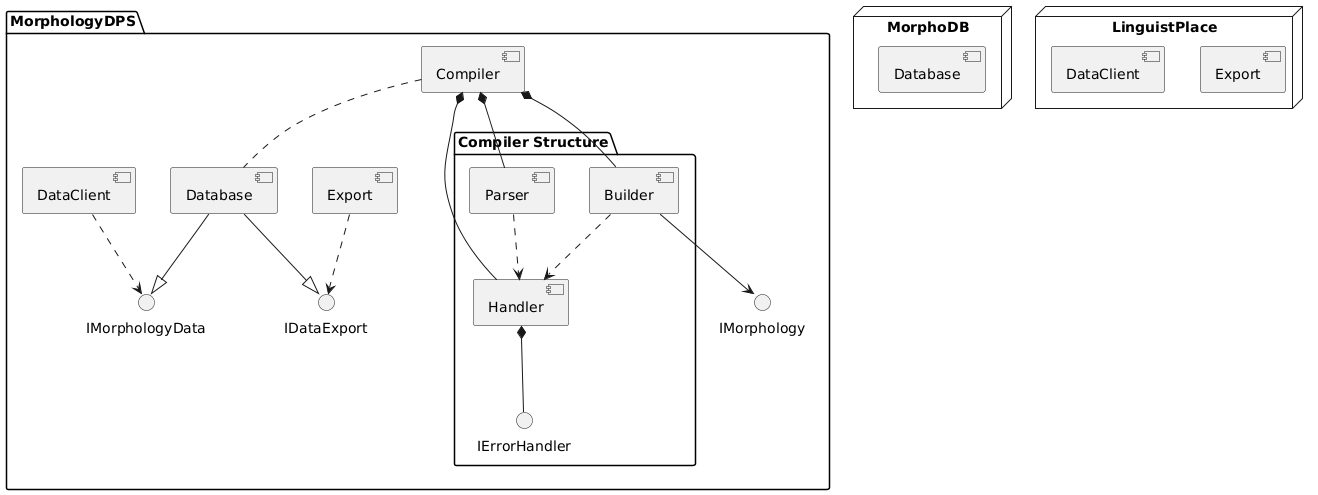
\includegraphics[width=\textwidth]{3.png}

\section{Задача 4}
Приложение класса Application содержит подключаемые модули. Подключаемый модуль класса Bean является либо процессным модулем ProcessBean, либо алгоритмическим модулем ComputeBean. Процессный модуль связан связью ComputeLink с подключаемыми модулями для выполнения расчетов.
\begin{itemize}
    \item Используя представление внутренней структуры, укажите, что специализация MainApp приложения Application включает один процессный модуль и два связанных с ним алгоритмических модуля.
    \item Доработайте модель, укажите, что приложение MainApp включает два связанных процессных модуля, один из которых является основным main.
    \item Покажите, что основной процессный модуль приложения MainApp реализует интерфейс управления вычислениями Computation, предоставляемый приложением через порт веб-сервисов ComputationEndpoint.
    \item Используя соединитель сборки, покажите, что основной процессный модуль приложения MainApp может обращаться через интерфейс Computation к приложению SecondApp.
    \item Перечислите все черты приложения MainApp (поведенческие, структурные, соединительные).
\end{itemize}

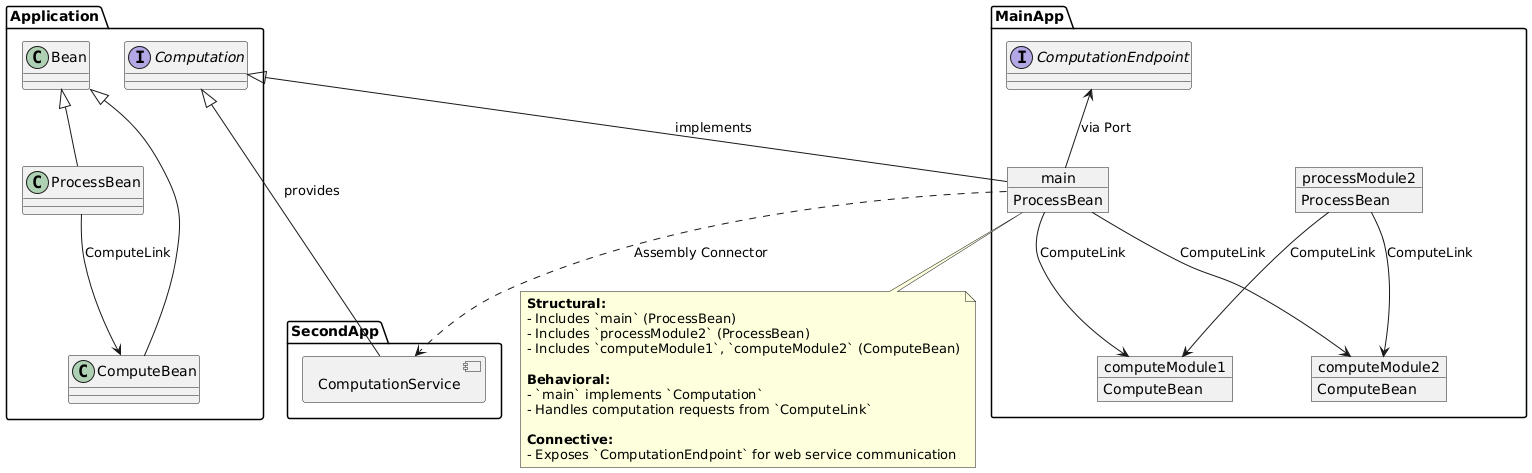
\includegraphics[width=\textwidth]{4.png}

\section{Задача 5}
Файл Morphology.dll материализует компонент MorphoEngine, который предоставляет интерфейс IMorphology. Компоненту MorphoEngine для работы необходим компонент RootObjects и файлы словарей. Файлы словарей имеют названия <ISO\_639-1\_код\_языка>.lng. Например, «ru.lng», «eng.lng». Компонент RootObjects материализован в библиотеке RootObject.dll.
\begin{itemize}
    \item Отобразите в модели артефакты и отношения между ними, необходимые для запуска морфологического модуля для работы с французским и немецким языками.
    \item Укажите, что для локализации сообщений пользователю, компонент MorphoEngine использует интерфейс IMorphoLocalize. Этот интерфейс уже реализован для русского и английского языков компонентами  MorphoLocalizeRu и MorphoLocalizeEn, материализованными библиотекой MorphoLocalize.dll. Добавьте в модель зависимость от компонента русской локализации.
    \item Проведите количественную оценку диаграммы.
    \item (*) Пометьте, что для корректной работы морфологическому модулю нужна библиотека RootObjects.dll версии 4.0.1.157.
    \item Указание: Так как атрибут «версия» не определен, нужно создать профиль, в котором добавить обязательное расширение метакласса Artifact в виде стереотипа VersionedArtifact. В этом расширении создать атрибут version типа String. Затем применить профиль к модели, используя отношение «apply» между пакетом, в котором размещена модель, и профилем. После этого указать версию библиотеки в теговом значении.
\end{itemize}

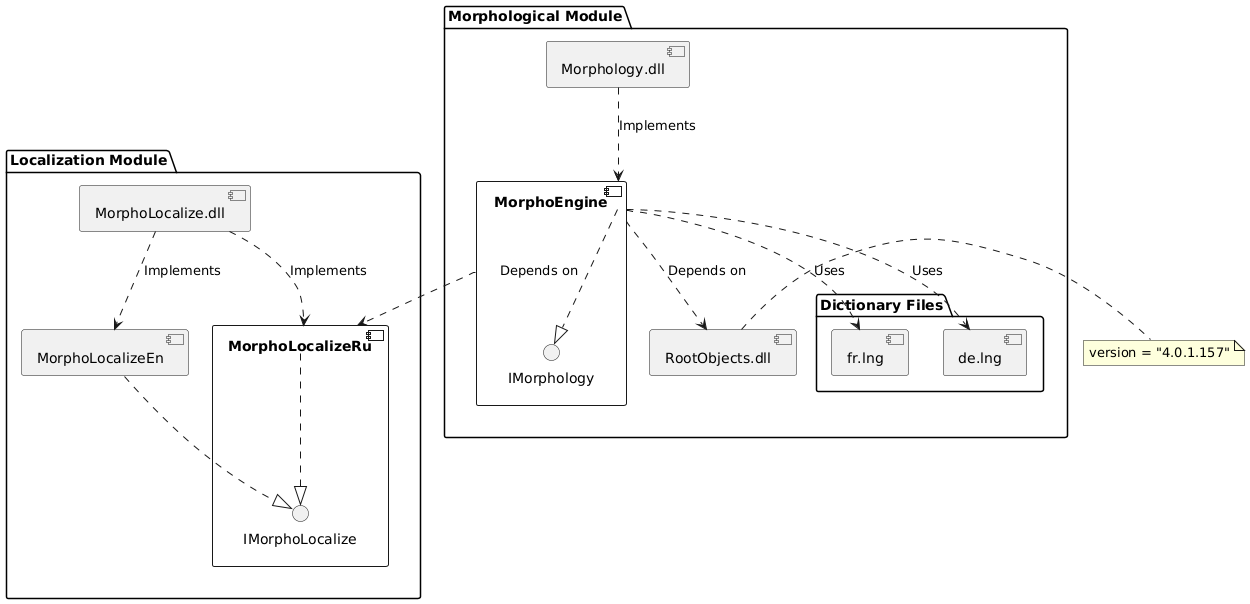
\includegraphics[width=\textwidth]{5.png}

Итоговая количественная оценка:
\begin{itemize}
    \item Общее количество элементов: 11
    \item Общее количество связей: 7
    \item Сложность: Низкая
\end{itemize}

\section*{Данные для расчета}

\begin{itemize}
    \item Оценка для элементов диаграммы (Sobj):
    \begin{itemize}
        \item Класс (class): 5
        \item Интерфейс (interface): 4
        \item Компонент (component): 4
        \item Примечание (note): 2
    \end{itemize}
    \item Оценка для связей на диаграмме (SLnk):
    \begin{itemize}
        \item Зависимость (dependency): 2
        \item Реализация (realization): 2
    \end{itemize}
    \item Число объектов на диаграмме (Obj): 6
    \item Число типов объектов на диаграмме (Tobj): 4
    \item Число типов связей на диаграмме (Tlnk): 2
\end{itemize}

\section*{Расчет}

$$S_{obj} = 5 + 4 + 4 + 2 = 15$$

$$S_{link} = 2 + 2 = 4$$

$$S = \frac{S_{obj} + S_{link}}{1 + Obj + \sqrt{T_{obj} + T_{link}}}$$

$$S = \frac{15 + 4}{1 + 6 + \sqrt{4 + 2}} 

$$S \approx \frac{19}{1 + 6 + 2.45} = \frac{19}{9.45} \approx 2.01$$

\end{document}
